\chapter{Canonical transformations}
\section{Point transformations}
Let's now focus on the possible transformations of coordinates.\\
In Lagrangian formalism a generic transformation is:
\begin{equation}
    \{q_{\alpha}\} \longrightarrow \{Q_{\alpha}\}\quad \text{s.t.}\quad Q_{\alpha} = Q_{\alpha}\brackets{q_1,q_2, \,\dots\, ,q_n,t}
\end{equation}
This is a \textbf{point transformation} in configuration space. We move from $n$ spatial coordinates to $n$ spatial coordinates.\\
In Hamiltonian formalism a generic transformation is:
\begin{equation}
    \begin{Bmatrix}
        q_{\alpha}\\[8pt]
        p_{\alpha}
    \end{Bmatrix} \longrightarrow
    \begin{Bmatrix}
        Q_{\alpha}\\[8pt]
        P_{\alpha}
    \end{Bmatrix}\quad \text{s.t.} \quad
    \begin{cases}
        Q_{\alpha} = Q_{\alpha}\brackets{q_1,q_2, \,\dots\, ,q_n,p_1,p_2, \,\dots\, ,p_n,t}\\[8pt]
        P_{\alpha} = P_{\alpha}\brackets{q_1,q_2, \,\dots\, ,q_n,p_1,p_2, \,\dots\, ,p_n,t}
    \end{cases}
\end{equation}
This is also a point transformation, but since we are in the phase space the new coordinates can be a mix of both $q_{\alpha}$ and $p_{\alpha}$. Now we can try to figure out if the relations found for $q_{\alpha}$ and $p_{\alpha}$ related to the Poisson brackets are also true for $Q_{\alpha}$ and $P_{\alpha}$.
We want:
\begin{equation}
    \begin{split}
        \pb{q_{\alpha}}{q_{\beta}} &= 0\\[8pt]
        \pb{p_{\alpha}}{p_{\beta}} &= 0\\[8pt]
        \pb{q_{\alpha}}{p_{\beta}} &= \delta_{\alpha \beta}
    \end{split} \implies
    \begin{split}
        \pb{Q_{\alpha}}{Q_{\beta}} &= 0\\[8pt]
        \pb{P_{\alpha}}{P_{\beta}} &= 0\\[8pt]
        \pb{Q_{\alpha}}{P_{\beta}} &= \delta_{\alpha \beta}
    \end{split}
\end{equation}
For example we want $\pb{Q_{\alpha}}{Q_{\beta}} = 0$. If we explicit the Poisson brackets we have:
\begin{equation}
    \pb{Q_{\alpha}}{Q_{\beta}} = \bigsum_{\gamma} \left(\pdv{Q_{\alpha}}{q_{\gamma}} \pdv{Q_{\beta}}{p_{\gamma}} - \pdv{Q_{\alpha}}{p_{\gamma}} \pdv{Q_{\beta}}{q_{\gamma}} \right)
\end{equation}
This is not always zero, therefore we will look for transformations such that:
\begin{equation}
    \begin{cases}
        \dot{Q}_{\alpha} = \pdv{\tilde{\hamfun}}{P_{\alpha}} \\[8pt]
        \dot{P}_{\alpha} = -\pdv{\tilde{\hamfun}}{Q_{\alpha}}
    \end{cases}
\end{equation}
Transformations that preserve those properties are called \textbf{canonical transformations}. The new Hamiltonian associated to those transformations is sometimes called \textit{k-Hamiltonian}.\\
In which condition this is true?\\
Recall that the \hamiltonref\;come from the \hpquotemath :
\begin{equation}
    \delta \action = \delta \int_{t_1}^{t_2}\lagr \dd{t} = \int_{t_1}^{t_2} \brackets{\bigsum_{\alpha}\dot{q}_{\alpha}p_{\alpha} - \hamfun} \dd{t} =0
\end{equation}
We want the same for the new Hamiltonian:
\begin{equation}
    \delta \tilde{\action} = \delta \int_{t_1}^{t_2}\tilde{\lagr} \dd{t} \int_{t_1}^{t_2} \brackets{\bigsum_{\alpha}\dot{Q}_{\alpha}P_{\alpha} - \tilde{\hamfun}} \dd{t} \overset{!}{=} 0
\end{equation}
\section{Generating functions}
We also know that the new Lagrangian and the old Lagrangian must describe the same system, and they have this relation:
\begin{equation}
    \lagr = \tilde{\lagr}+\dv{F}{t}
\end{equation}
So there must exist a function $F$ such that this is true for a transformation to be canonical. These functions are called \textbf{generating functions}.
In principle a generic $F$ can depend on both the old and the new coordinates:
\begin{equation}
    F = F(\vec{q},\vec{p},\vec{Q},\vec{P},t)
\end{equation}
But if all the coordinates were independent we would have $4n$ variables plus time. The maximum number of variables is $2n$ hence there must be at least $2n$ dependent variables.\\
If we know the expression for both the generating function and the transformation equations we are done. This of course is not the interesting case. We can reconstruct the transformation equations just from the expression of $F$. We can distinguish 4 categories of generating functions:
\begin{enumerate}
    \item $F_1 = F_1(\vec{q},\vec{Q},t)$ (\nth{1} type functions)
    \item $F_2 = F_2(\vec{q},\vec{P},t)$ (\nth{2}  type functions)
    \item $F_3 = F_3(\vec{p},\vec{Q},t)$ (\nth{3}  type functions)
    \item $F_4 = F_4(\vec{p},\vec{P},t)$ (\nth{4}  type functions)
\end{enumerate}
From the relation between the Lagrangians we have:
\begin{equation}
    \begin{split}
        \lagr &= \tilde{\lagr}+\dv{F}{t}\\[8pt]
        \bigsum_{\alpha}p_{\alpha}\dd{q_{\alpha}} - \hamfun\dd{t} &= \bigsum_{\alpha}P_{\alpha}\dd{Q_{\alpha}} - \tilde{\hamfun}\dd{t} + \dd{F}\\[8pt]
        &\Downarrow \\[8pt]
        \dd{F} = \bigsum_{\alpha}p_{\alpha}\dd{q_{\alpha}} &- \bigsum_{\alpha}P_{\alpha}\dd{Q_{\alpha}} + \brackets{\tilde{\hamfun}- \hamfun}\dd{t}\\[8pt]
        &\Downarrow \\[8pt]
        F &= F(\vec{q},\vec{Q})
    \end{split}
\end{equation}
This means that the generating function in the relation with the Lagrangians is a first type function $F = F_1$. In this case the differential of $F_1$ is:
\begin{equation}
    \dd{F_1} = \bigsum_{\alpha} \pdv{F_1}{q_{\alpha}} \dd{q_{\alpha}} + \bigsum_{\alpha} \pdv{F_1}{Q_{\alpha}} \dd{Q_{\alpha}} + \pdv{F_1}{t} \dd{t}
\end{equation}
And so we get:
\begin{equation} \label{F1_Canonical}
    \begin{cases}
        \pdv{F_1}{q_{\alpha}} = p_{\alpha}\\[8pt]
        \pdv{F_1}{Q_{\alpha}} = -P_{\alpha}\\[8pt]
        \pdv{F_1}{t} = \brackets{\tilde{\hamfun}- \hamfun}
    \end{cases}
\end{equation}
Hence:
\begin{equation}
    \begin{cases}
        p = p(\vec{q},\vec{Q},t)\\[8pt]
        P = P(\vec{q},\vec{Q},t)
    \end{cases}
\end{equation}
By inverting the first equation we can get:
\begin{equation}
    Q = Q(\vec{q},\vec{p},t)\\[8pt]
\end{equation}
Substituting this into the second equation we finally get the transformation equations:
\begin{equation}
    \begin{cases}
        Q = Q(\vec{q},\vec{p},t)\\[8pt]
        P = P(\vec{q},\vec{p},t)
    \end{cases}
\end{equation}
Also from the third equation in \eqref{F1_Canonical} we have:
\begin{equation}
    \tilde{\hamfun} = \hamfun + \pdv{F_1}{t}
\end{equation}
And so if $F_1$ does not depend on time explicitly:
\begin{equation}
    \tilde{\hamfun} = \hamfun
\end{equation}
This means that the Hamiltonians are equal, but we need to keep in mind that $\tilde{\hamfun}$ depends on the new coordinates so if we have a generic $\hamfun$ substituting $Q$ and $P$ instead of $q$ and $p$ \underline{does not} give $\tilde{\hamfun}$. For example:
\begin{equation}
    \hamfun = \dfrac{p^2}{2m} + \dfrac{\alpha}{q} \notimplies \tilde{\hamfun} = \dfrac{P^2}{2m} + \dfrac{\alpha}{Q}
\end{equation}
Instead we need to substitute the expression of the old coordinates in terms of the new one (or viceversa if we have $\tilde{\hamfun}$).\\
Now let $F$ be a generating function of the first type but with:
\begin{equation}
    \begin{cases}
        Q = q\\[8pt]
        P = P(\vec{q},\vec{p},t)
    \end{cases}
\end{equation}
Then $q$ and $Q$ are not independent, therefore we should have only $n$ independent variables in $F$, but this is not what we want. In order to write $F$ in terms of only independent coordinates we must find a way to express $F$ as a second type function:
\begin{equation}
    F_1(\vec{q},\vec{Q},t) \longrightarrow F_2(\vec{q},\vec{P},t)
\end{equation}
This is just an application of the Legendre transformations:
\begin{equation}
    \begin{split}
        \dd{F_1} &= \bigsum_{\alpha}p_{\alpha}\dd{q_{\alpha}} - \bigsum_{\alpha}P_{\alpha}\dd{Q_{\alpha}} + \brackets{\tilde{\hamfun}- \hamfun}\dd{t}\\[8pt]
        \dd{\brackets{F_1 + \bigsum_{\alpha}P_{\alpha}Q_{\alpha}}} &= \bigsum_{\alpha}p_{\alpha}\dd{q_{\alpha}}  + \bigsum_{\alpha}Q_{\alpha}\dd{P_{\alpha}} + \brackets{\tilde{\hamfun}- \hamfun}\dd{t}
    \end{split}
\end{equation}
And so:
\begin{equation}
    F_2 = F_1 + \bigsum_{\alpha}P_{\alpha}Q_{\alpha}
\end{equation}
From this, we obtain the relations:
\begin{equation}
    \begin{cases}
        \pdv{F_2}{q_{\alpha}} = p_{\alpha}\\[8pt]
        \pdv{F_2}{P_{\alpha}} = Q_{\alpha}\\[8pt]
        \pdv{F_2}{t} = \pdv{F_1}{t}
    \end{cases}
\end{equation}
As for the first type this means that:
\begin{equation}
    \begin{cases}
        p = p(\vec{q},\vec{P},t)\\[8pt]
        Q = P(\vec{q},\vec{P},t)
    \end{cases}
\end{equation}
By inverting the first equation we can get:
\begin{equation}
    P = P(\vec{q},\vec{p},t)
\end{equation}
Substituting this into the second equation we get the transformation equations:
\begin{equation}
    \begin{cases}
        Q = Q(\vec{q},\vec{p},t)\\[8pt]
        P = P(\vec{q},\vec{p},t)
    \end{cases}
\end{equation}
Similarly we can find a way to express $F_1$ as a third type function $F_3$. This is again an application of the Legendre transformations:
\begin{equation}
    \begin{split}
        \dd{F_1} = \bigsum_{\alpha}p_{\alpha}\dd{q_{\alpha}} - \bigsum_{\alpha}P_{\alpha}\dd{Q_{\alpha}} + \brackets{\tilde{\hamfun}- \hamfun}\dd{t}\\
    \dd{\brackets{F_1 - \bigsum_{\alpha}q_{\alpha}p_{\alpha}}} = -\bigsum_{\alpha}q_{\alpha}\dd{p_{\alpha}} - \bigsum_{\alpha}P_{\alpha}\dd{Q_{\alpha}} + \brackets{\tilde{\hamfun}- \hamfun}\dd{t}
    \end{split}
\end{equation}
And so:
\begin{equation}
    F_3 = F_1 - \bigsum_{\alpha}q_{\alpha}p_{\alpha}
\end{equation}
From this, we obtain the relations:
\begin{equation}
    \begin{cases}
        \pdv{F_3}{p_{\alpha}} = -q_{\alpha}\\[8pt]
        \pdv{F_3}{Q_{\alpha}} = -P_{\alpha}\\[8pt]
        \pdv{F_3}{t} = \pdv{F_1}{t}
    \end{cases}
\end{equation}
As for the first type, this means that:
\begin{equation}
    \begin{cases}
        q = q(\vec{p},\vec{Q},t)\\[8pt]
        P = P(\vec{p},\vec{Q},t)
    \end{cases}
\end{equation}
By inverting the first equation, we can get:
\begin{equation}
    Q = Q(\vec{q},\vec{p},t)
\end{equation}
Substituting this into the second equation, we get the transformation equations:
\begin{equation}
    \begin{cases}
        Q = Q(\vec{q},\vec{p},t)\\[8pt]
        P = P(\vec{q},\vec{p},t)
    \end{cases}
\end{equation}
Finally we can find a way to express $F_1$ as a fourth type function $F_4$. This is a double application of the Legendre transformations (we can think to pass through second type first or third type first and then go to fourth type):
\begin{equation}
    \begin{split}
        \dd{F_1} &= \bigsum_{\alpha}p_{\alpha}\dd{q_{\alpha}} - \bigsum_{\alpha}P_{\alpha}\dd{Q_{\alpha}} + \brackets{\tilde{\hamfun}- \hamfun}\dd{t}\\
        \dd{\brackets{F_1 + \bigsum_{\alpha}P_{\alpha}Q_{\alpha} - \bigsum_{\alpha}q_{\alpha}p_{\alpha}}} &= -\bigsum_{\alpha}q_{\alpha}\dd{p_{\alpha}} + \bigsum_{\alpha}Q_{\alpha}\dd{P_{\alpha}} + \brackets{\tilde{\hamfun}- \hamfun}\dd{t}
    \end{split}
\end{equation}
And so:
\begin{equation}
    F_4 = F_1 + \bigsum_{\alpha}P_{\alpha}Q_{\alpha} - \bigsum_{\alpha}q_{\alpha}p_{\alpha}
\end{equation}
From this, we obtain the relations:
\begin{equation}
    \begin{cases}
        \pdv{F_4}{p_{\alpha}} = -q_{\alpha}\\[8pt]
        \pdv{F_4}{P_{\alpha}} = Q_{\alpha}\\[8pt]
        \pdv{F_4}{t} = \pdv{F_1}{t}
    \end{cases}
\end{equation}
As for the first type, this means that:
\begin{equation}
    \begin{cases}
        q = q(\vec{p},\vec{P},t)\\[8pt]
        Q = Q(\vec{p},\vec{P},t)
    \end{cases}
\end{equation}
By inverting the first equation, we can get:
\begin{equation}
    P = P(\vec{q},\vec{p},t)
\end{equation}
Substituting this into the second equation, we get the transformation equations:
\begin{equation}
    \begin{cases}
        Q = Q(\vec{q},\vec{p},t)\\[8pt]
        P = P(\vec{q},\vec{p},t)
    \end{cases}
\end{equation}
\section{Poisson brackets and canonical transformations}
As we anticipated before we want to know how the Poisson brackets act on the new coordinates. In particular, we state this theorem:
\begin{theorem}{}
  A transformation is canonical if and only if the canonical Poisson brackets are invariant
\end{theorem}
This means that they are the same in the old and new coordinates. For example:
\begin{equation}
    \pb{Q_{\alpha}}{P_{\beta}}_{QP} = \delta_{\alpha \beta} \implies \pb{Q_{\alpha}}{P_{\beta}}_{qp} = \delta_{\alpha \beta}
\end{equation}
The subscript represents in respect to what coordinates we are calculating the Poisson brackets. This theorem also as an important corollary:
\begin{corollary}{}
    If the canonical Poisson brackets are invariant then all Poisson brackets are invariant
\end{corollary}
Which means that for any functions $f$ and $g$ in the phase space:
\begin{equation}
    \pb{f}{g}_{QP} = \pb{f}{g}_{qp} = \pb{f}{g}
\end{equation}
In the last notation (which is the usual one) we do not specify the coordinates since it makes no difference.\\
Another relation that is true in general is:
\begin{equation}
    \dv{f}{t} = \pb{f}{\hamfun} + \pdv{f}{t}
\end{equation}
If we are dealing with a function that is also a constant of the motion then:
\begin{equation}
    \pb{f}{\hamfun} = - \pdv{f}{t}
\end{equation}
If this function also does not depend on time explicitly:
\begin{equation}
    \pb{f}{\hamfun} = 0
\end{equation}
\section{Examples}
We will now show some examples of the application of the Legendre transformations and in general of the utility of the generating functions.
\subsection{Ex. 1}
Given a generating function of the first type $F_1 = F_1(\vec{q},\vec{Q},t)$ such that:
\begin{equation}
    F_1 = \bigsum_{\alpha} q_{\alpha}Q_{\alpha}
\end{equation}
By applying \hamiltonref\;and Legendre transformations we get:
\begin{equation}
    \begin{cases}
        Q_{\beta} = \pdv{F_1}{q_{\beta}} = p_{\beta}\\[8pt]
        q_{\beta} = \pdv{F_1}{Q_{\beta}} = -P_{\beta}
    \end{cases}
\end{equation}
And so the transformation equations are:
\begin{equation}
    \begin{cases}
        Q_{\alpha} = p_{\alpha}\\[8pt]
        P_{\alpha} = -q_{\alpha}
    \end{cases}
\end{equation}
So this transformation just swaps the momentum and the position coordinates (taking into account some sign changes).
\subsection{Ex. 2}
Given a generating function of the second type $F_2 = F_2(\vec{q},\vec{P},t)$ such that:
\begin{equation}
    F_2 = \bigsum_{\alpha} q_{\alpha}P_{\alpha}
\end{equation}
By applying \hamiltonref\;and Legendre transformations we get:
\begin{equation}
    \begin{cases}
        P_{\beta} = \pdv{F_2}{q_{\beta}} = p_{\beta}\\[8pt]
        q_{\beta} = \pdv{F_2}{P_{\beta}} = Q_{\beta}
    \end{cases}
\end{equation}
And so the transformation equations are:
\begin{equation}
    \begin{cases}
        Q_{\alpha} = q_{\alpha}\\[8pt]
        P_{\alpha} = p_{\alpha}
    \end{cases}
\end{equation}
So this transformation is the \textbf{identity transformation} since the new momenta and positions are equal to the old ones.
\begin{equation}
    \underset{\text{Identity}}{\boxed{F_2 = \bigsum_{\alpha} q_{\alpha}P_{\alpha}}}
\end{equation}
\subsection{Ex. 3}
Given a generating function of the second type $F_2 = F_2(\vec{q},\vec{P},t)$ such that:
\begin{equation}
    F_2 = \bigsum_{\alpha} f_{\alpha}(\vec{q},t) P_{\alpha}
\end{equation}
By applying \hamiltonref\;and Legendre transformations we get:
\begin{equation}
    \begin{split}
        p_{\beta} = \pdv{F_2}{q_{\beta}} =  \,\dots\, \\[8pt]
        Q_{\beta} = \pdv{F_2}{P_{\beta}} = f_{\beta}(\vec{q},t)
    \end{split}
\end{equation}
So new positions only depend on old positions, hence this is actually a point transformation in configuration space. This is why any point transformation in configuration space is always canonical.
\subsection{Ex. 4}
Now let the Hamiltonian of a system be:
\begin{equation}
    \hamfun = \dfrac{p^2}{2m} + mgq
\end{equation}
\hamiltonref\;give:
\begin{equation}
    \begin{cases}
        \dot{q} = \pdv{\hamfun}{p} = \dfrac{p}{m}\\[8pt]
        \dot{p} = -\pdv{\hamfun}{q} = -mg
    \end{cases}
\end{equation}
Those are just the Newton's equations for a particle in the gravitational potential. Now let's make a transformation:
\begin{equation}
    F_1 = -\dfrac{Q}{q}
\end{equation}
From this we get:
\begin{equation}
    \begin{cases}
        p = \pdv{F_1}{q} = \dfrac{Q}{q^2}\\[8pt]
        P = -\pdv{F_1}{Q} = \dfrac{1}{q}
    \end{cases}
\end{equation}
From this getting the transformation equations is trivial:
\begin{equation}
    \begin{cases}
        Q = pq^2\\[8pt]
        P = \dfrac{1}{q}
    \end{cases}
\end{equation}
We can invert these relations:
\begin{equation}
    \begin{cases}
        q = \dfrac{1}{P}\\[8pt]
        p = QP^2
    \end{cases}
\end{equation}
And if we substitute back into the old Hamiltonian we get the new expression:
\begin{equation}
    \tilde{\hamfun} = \dfrac{P^4 Q^2}{2m} + \dfrac{mg}{P}
\end{equation}
This again shows that to get the new Hamiltonian we cannot just substitute $Q$ instead of $q$ and $P$ instead of $p$.\\
Also for the new Lagrangian we have:
\begin{equation}
    \begin{split}
        \lagr &= \tilde{\lagr} + \dv{F_1}{t} =\\[8pt]
        &= \tilde{\lagr} + \dv{}{t}\brackets{-QP} =\\[8pt]
        &=\tilde{\lagr} - \dot{Q}P - Q\dot{P}
    \end{split}
\end{equation}
Which gives:
\begin{equation}
    \tilde{\lagr} = \lagr + \dot{Q}P + Q\dot{P}
\end{equation}
We want to check that this is a canonical transformation. We can do this by calculating the canonical Poisson brackets in the new and old coordinates. For the new ones:
\begin{equation}
    \begin{split}
        \pb{Q}{P}_{QP} &= \left(\pdv{Q}{Q} \pdv{P}{P} - \cancel{\pdv{Q}{P}} \cancel{\pdv{P}{Q}} \right) = 1\\[8pt]
        \pb{Q}{Q}_{QP} &= \left(\pdv{Q}{Q} \cancel{\pdv{Q}{P}} - \cancel{\pdv{Q}{P}} \pdv{Q}{Q} \right) = 0\\[8pt]
        \pb{P}{P}_{QP} &= \left(\cancel{\pdv{P}{Q}} \pdv{P}{P}  -  \pdv{P}{P} \cancel{\pdv{P}{Q}}\right) = 0
    \end{split}
\end{equation}
For the old ones:
\begin{equation}
    \begin{split}
        \pb{Q}{P}_{qp} &= \left(\pdv{Q}{q} \pdv{P}{p} - \pdv{Q}{p} \pdv{P}{q} \right) = \\[8pt]
        &= \left(\pdv{}{q}(pq^2) \cancel{\pdv{}{p}\left(\dfrac{1}{q}\right)} - \pdv{}{p}(pq^2) \pdv{}{q}\left(\dfrac{1}{q}\right) \right) = \\[8pt]
        &= \left(- q^2  \left(-\dfrac{1}{q^2}\right) \right) = 1
    \end{split}
\end{equation}
\begin{equation}
    \begin{split}
        \pb{Q}{Q}_{qp} &= \left(\pdv{}{q}(pq^2) \pdv{}{p}(pq^2) - \pdv{}{p}(pq^2) \pdv{}{q}(pq^2) \right) = \\[8pt]
        &= \left(2pq  q^2 - q^2  2pq \right) = 0
    \end{split}
\end{equation}
\begin{equation}
    \begin{split}
        \pb{P}{P}_{qp} &= \bigsum_{\alpha} \left(\pdv{P}{q_{\alpha}} \pdv{P}{p_{\alpha}} - \pdv{P}{p_{\alpha}} \pdv{P}{q_{\alpha}} \right) = \\[8pt]
        &= \left(\pdv{}{q}\left(\dfrac{1}{q}\right) \cancel{\pdv{}{p}\left(\dfrac{1}{q}\right)} - \cancel{\pdv{}{p}\left(\dfrac{1}{q}\right)} \pdv{}{q}\left(\dfrac{1}{q}\right) \right) = 0
    \end{split}
\end{equation}
And so we verified that the canonical Poisson brackets are invariant.
\subsection{Ex. 5}
Now given a transformation we want to prove that it is a canonical transformation:
\begin{equation}
    \begin{cases}
        Q = \ln \brackets{\dfrac{p}{q}}\\[8pt]
        P = \brackets{-\dfrac{q^2}{2}-1}\dfrac{p}{1}
    \end{cases}
\end{equation}
We have two methods:\\
The \textbf{first method} will just be calculating all the Poisson brackets and verifying that they are invariant.\\
The Poisson brackets in the new coordinates will always be trivial:
\begin{equation}
    \begin{split}
        \pb{Q}{P}_{QP} &= 1\\[8pt]
        \pb{Q}{Q}_{QP} &= 0\\[8pt]
        \pb{P}{P}_{QP} &= 0
    \end{split}
\end{equation}
Now we can evaluate the Poisson brackets with respect to the old coordinates:
\begin{equation}
    \begin{split}
        \pb{Q}{P}_{qp} &= \left(\pdv{Q}{q} \pdv{P}{p} - \pdv{Q}{p} \pdv{P}{q} \right) = \\[8pt]
        &= \bbrackets{\pdv{}{q}\left(\ln\brackets{\dfrac{p}{q}}\right) \pdv{}{p}\left(\brackets{-\dfrac{q^2}{2}-1}\dfrac{p}{q}\right) -\\[8pt]
        &- \pdv{}{p}\left(\ln\brackets{\dfrac{p}{q}}\right) \pdv{}{q}\left(\brackets{-\dfrac{q^2}{2}-1}\dfrac{p}{q}\right) } = \\[8pt]
        &= \left(-\dfrac{1}{q}  \brackets{-\dfrac{q^2}{2}-1}  \dfrac{1}{q} - \dfrac{1}{p}  \brackets{-q  \dfrac{p}{q} + \brackets{-\dfrac{q^2}{2}-1}  \dfrac{1}{q}} \right) = \\[8pt]
        &= \left(\cancel{\dfrac{\dfrac{q^2}{2} + 1}{q^2}} + 1 - \cancel{\dfrac{\dfrac{q^2}{2} + 1}{q^2}} \right) = 1
    \end{split}
\end{equation}
The other ones are trivial:
\begin{equation}
    \pb{Q}{Q}_{qp} = \left(\pdv{Q}{q} \pdv{Q}{p} - \pdv{Q}{p} \pdv{Q}{q} \right) = 0
\end{equation}
\begin{equation}
    \pb{P}{P}_{qp} = \left(\pdv{P}{q} \pdv{P}{p} - \pdv{P}{p} \pdv{P}{q} \right) = 0
\end{equation}

\section{Active canonical transformations}
Up to now we used ``passive'' transformations, which means that the transformation does not affect the state of the system. Instead, now we will make use of \textbf{active transformations} which are transformations that do not change the axes, but they change the state of the system.\\
First we need to introduce a new definition:
\begin{definition}{Infinitesimal canonical transformations}
    Are transformations that differ from the identity transformation for an infinitesimal amount.
\end{definition}
This definition is equivalent to:
\begin{equation}
    F_2 = \bigsum_{\alpha} q_{\alpha}P_{\alpha} + \varepsilon G(\vec{q},\vec{P},t)
\end{equation}
And so we have:
\begin{equation}
    \begin{cases}
        p_{\gamma} = \pdv{F_2}{q_{\gamma}} = P_{\gamma} + \varepsilon\pdv{ G}{q_{\gamma}}\\[8pt]
        Q_{\gamma} = \pdv{F_2}{P_{\gamma}} = Q_{\gamma} + \varepsilon\pdv{ G}{P_{\gamma}}
    \end{cases}
\end{equation}
The term depending on the function $G$ are the infinitesimal changes. Let us define:
\begin{equation}
    \begin{split}
        \delta p_{\gamma} &\defineeq -\varepsilon\pdv{ G}{q_{\gamma}}\\[8pt]
        \delta q_{\gamma} &\defineeq \varepsilon\pdv{ G}{P_{\gamma}}
    \end{split}
\end{equation}
We want to substitute the partial derivative of $G$ with respect to $P_{\gamma}$ with the partial derivative of $G$ with respect to $p_{\gamma}$:
\begin{equation}
    \pdv{G}{p_{\gamma}} = \bigsum_{\alpha} \brackets{\pdv{G}{P_{\alpha}}\pdv{P_{\alpha}}{p_{\gamma}} + \pdv{G}{q_{\alpha}}\cancel{\pdv{q_{\alpha}}{p_{\gamma}}}}
\end{equation}
So from the equation of the generating function:
\begin{equation}
    \begin{split}
        \pdv{P_{\alpha}}{p_{\gamma}} &= \pdv{}{p_{\gamma}}\brackets{p_{\alpha} - \varepsilon\pdv{ G}{q_{\alpha}}} = \\[8pt]
        &= \delta_{\alpha \gamma} - \underbrace{\varepsilon\pdv{ G}{q_{\alpha}}}_{\text{infinitesimal}}
    \end{split}
\end{equation}
The term underlined is infinitesimal and can be disregarded. This leads to:
\begin{equation}
    \pdv{G}{p_{\gamma}} = \bigsum_{\alpha} \pdv{G}{P_{\alpha}}\delta_{\alpha \gamma} = \pdv{G}{P_{\gamma}}
\end{equation}
Now let's define a new vector containing all the coordinates and momenta:
\begin{equation}
    \vec{\eta} \defineeq \begin{pmatrix}
        q_1\\[8pt] \,\dots\, \\[8pt]q_n\\[8pt]p_1\\[8pt] \,\dots\, \\[8pt]p_n
    \end{pmatrix}
    \quad n+n = 2n \quad \text{elements}
\end{equation}
In this way we can write in a compact form:
\begin{equation}
    \delta \vec{\eta} = \varepsilon \pb{\eta}{G}
\end{equation}
Where, by using the Poisson brackets on the vector we mean that we apply them between every component and $G$. Let's for example choose a particular form of $G$:
\begin{equation}
    G = p_i
\end{equation}
Then only the $q_i$ component of the vector $\delta \vec{\eta}$ has value, the rest of the components are zero:
\begin{equation}
    \delta \vec{\eta} = \begin{pmatrix}
        0\\[8pt] \,\dots\, \\[8pt]\varepsilon\\[8pt]0\\[8pt] \,\dots\, \\[8pt]0
    \end{pmatrix}
\end{equation}
What if $q_i$ is a collective coordinate? Let's take for example $x_{CM}$ then $p_i = P_x$ which is the $x$ component of the total linear momentum. $P_x$ generates a translation of the system as a whole along the $x$ axis. In general $\vec{P}$ generates a translation along his direction (in real space). Let's also notice that if $q_i = x_{CM}$ is a collective coordinate and is cyclic then its corresponding momentum $p_i = P_x$ is conserved and also:
\begin{equation}
  \pdv{\hamfun}{x_{CM}}=0
\end{equation}
Therefore $\hamfun$ does not change. Every conserved quantity is the generator of an infinitesimal displacement that does not change the Hamiltonian. Let's make another example.\\
Let us now consider an angular coordinate $q_i$ such that the associated momentum $p_i$ is a rotation of the system as a whole. If $q_i$ is also cyclic then the Hamiltonian is invariant to rotations along the axis of rotation identified by $p_i$. To make a more concrete example we take $q_i = \theta$ such that $\theta$ is cyclic and $p_i = L_z$, then the Hamiltonian is invariant with respect to rotations along the $z$ axis.\\
Now instead let's take another specific form of the function $G$ in particular let's say that $G= \hamfun$, then:
\begin{equation}
  \delta \vec{\eta} = \varepsilon\pb{\eta}{\hamfun} = \varepsilon\dv{\vec{\eta}}{t}
\end{equation}
And also:
\begin{equation}
  \begin{split}
      \delta p_{\alpha} &\defineeq -\varepsilon\pdv{\hamfun}{q_{\alpha}} = \varepsilon \dot{p}_{\alpha}\\[8pt]
      \delta q_{\alpha} &\defineeq \varepsilon\pdv{\hamfun}{P_{\alpha}} = \varepsilon \dot{q}_{\alpha}
  \end{split}
\end{equation}
If we have a function $[F_2] = \unit{\joule  \cdot \second}$ then $F_2$ will be in the form:
\begin{equation}
  F_2 = \bigsum_{\alpha}\brackets{ \,\dots\, } + \varepsilon \hamfun
\end{equation}
And so the infinitesimal term $\varepsilon$ is an infinitesimal displacement in time. And so we can understand that the Hamiltonian is the generator of the infinitesimal time evolution.\\
Now let's notice one more thing about the Hamiltonian. If we let the Hamiltonian be the generating function we can either have $\hamfun$ to be explicitly depend on time or not. If $\hamfun$ does depend on time explicitly then:
\begin{equation}
  \dv{\hamfun}{t} = \cancel{\pb{\hamfun}{\hamfun}} + \pdv{\hamfun}{t} \quad \implies \quad  \dv{\hamfun}{t} = \pdv{\hamfun}{t}
\end{equation}
And so the transformation generated by the Hamiltonian changes the Hamiltonian itself. Instead, if $\hamfun$ does not depend on time explicitly:
\begin{equation}
  \dv{\hamfun}{t} = 0
\end{equation}
Which means that the Hamiltonian is a constant of the motion and the transformation leave $\hamfun$ unaffected.\\
Let us now consider a generic function $u(q,p,t)$ in the phase space such that $u$ does not depend on time explicitly. Then we can state that:
\begin{equation}
  \dv{u}{t} = \pb{u}{\hamfun} + \cancel{\pdv{u}{t}} \quad \implies \quad  \dv{u}{t} = \pb{u}{\hamfun}
\end{equation}
We now express $u$ as dependent on time, but we know that its ``dependence'' on time is due to $q$ and $p$ and instead time does not directly appear in the equation fo $u$. And so for an infinitesimal time change we have:
\begin{equation}
  u(t+\dd{t}) - u(t) = \dot{u}\dd{t}
\end{equation}
Since we know what the time derivative of $u$ is we have:
\begin{equation}
  u(t+\dd{t}) - u(t) = \pb{u}{\hamfun}
\end{equation}
So to reconstruct the time evolution of $u$ we just need to know the time evolution of the Hamiltonian. Keep in mind that $u$ is just a generic function, so this argument is valid for any function with the same properties as $u$.
\begin{figure}[H]
  \centering
  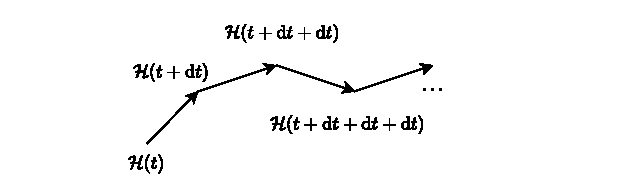
\includegraphics[width=0.6\textwidth]{res/svg/hamiltonian_time_evolution.drawio}
  \caption{Time evolution through Hamiltonian}
\end{figure}
In particular, we can write the Taylor expansion of $u$ and get:
\begin{equation}
  u(t) = u(t_0) + \dv{u}{t}\bigg|_{t_0} (t - t_0) + \frac{1}{2!} \dv[2]{u}{t}\bigg|_{t_0} (t - t_0)^2 +  \,\dots\,
\end{equation}
We can express the multiple derivatives as:
\begin{equation}
  \begin{split}
    \dv{u}{t} &= \pb{u}{\hamfun}\\[8pt]
    \dv[2]{u}{t} &= \pb{\pb{u}{\hamfun}}{\hamfun}\\[8pt]
    \dv[3]{u}{t} &= \pb{\pb{\pb{u}{\hamfun}}{\hamfun}}{\hamfun}\\[8pt]
    & \,\dots\,
  \end{split}
\end{equation}
We then define the operator $\hat{H}$ such that:
\begin{equation}
  \hat{H} = \pb{}{\hamfun}
\end{equation}
And so we can write the Taylor series as:
\begin{equation}
  \begin{split}
    u(t) &= u(t_0) + \hat{H}u(t)\bigg|_{t_0} (t - t_0) + \frac{1}{2!} \hat{H}^2u(t)\bigg|_{t_0} (t - t_0)^2 +  \,\dots\,  =\\[8pt]
    &= \bigsum_{k=0}^\infty \dfrac{1}{k!} \hat{H}^k u(t)\bigg|_{t_0}(t - t_0)^k =\\[8pt]
    &= u(t_0)\bigsum_{k=0}^\infty \dfrac{1}{k!} \hat{H}^k (t - t_0)^k \defineeq u(t_0) \efunction^{\brackets{t-t_0}\hat{H}}
  \end{split}
\end{equation}
Keep in mind that the last step is more of a ``definition'' consistent with the fact that we would get exactly the Taylor series of the exponential if we replaced $\hat{H}$ with a usual variable.
This formula is the classical counterpart of the quantum mechanical ``propagator''. In particular, we notice that in both cases the formula contains the Hamiltonian (the operator made from the Poisson brackets in the classical case and the operator associated to the Hamiltonian in the quantum case) and also that both are used to get the time evolution of something.
